\chapter{Configuration Wi-Fi}
Le Wi-Fi est désactivé en fonctionnement normal. Pendant la configuration, placer le téléphone à environ 10–20 cm de l'indicateur. Le mot de passe par défaut est 1234567890 et le panneau est accessible à http://192.168.4.1.

USB étant débranché, mettre le contact ou l'alimentation puis appuyer immédiatement sur le bouton arrière. Un code QR apparaît. Désactiver les données mobiles, scanner le code et connecter le téléphone au réseau Wi-Fi de l'indicateur. Ouvrir le panneau dans le navigateur, choisir l'application et le capteur adapté, enregistrer puis couper et remettre le contact.

En cas d'échec, rapprocher le téléphone et vérifier qu'il reste connecté au réseau de l'indicateur malgré l'absence d'Internet. Répéter si nécessaire le démarrage en mode QR. Le bouton arrière permet aussi d'interagir avec les applications et de choisir le mode de démarrage lors de la programmation initiale.

USB est prévu pour la programmation initiale ; l'interface web est recommandée pour les mises à jour suivantes. Déconnecter tous les fils du véhicule avant d'utiliser USB. Suivre les instructions du micrologiciel concerné ; la source ne décrit ni procédure de récupération ni menu de téléversement.

\begin{figure}[H]
\centering
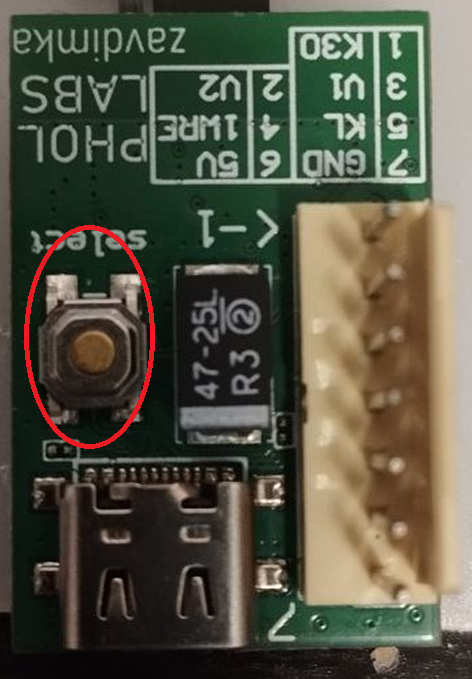
\includegraphics[width=.85\textwidth,height=.60\textheight,keepaspectratio]{figures/ivevo/image11.png}
\caption{Configuration Wi-Fi}
\end{figure}
